% R_V Paper - Main LaTeX Document
% "Coordinated Dual-Space Geometric Transformations Mediate Recursive Self-Reference in Transformer Value Spaces"
% Template: ICLR 2026 format
% Last updated: 2026-02-04

\documentclass{article}

% Required packages
\usepackage[utf8]{inputenc}
\usepackage[T1]{fontenc}
\usepackage{graphicx}
\usepackage{amsmath,amssymb,amsfonts}
\usepackage{booktabs}
\usepackage{natbib}
\usepackage{hyperref}
\usepackage{microtype}
\usepackage{xcolor}

% Page setup (adjust for target venue)
\usepackage[margin=1in]{geometry}

% Graphics path
\graphicspath{{figures/}}

% Custom commands
\newcommand{\RV}{R_V}
\newcommand{\Vpar}{V_\parallel}
\newcommand{\Vperp}{V_\perp}
\newcommand{\PR}{\text{PR}}

\title{Coordinated Dual-Space Geometric Transformations Mediate Recursive Self-Reference in Transformer Value Spaces}

\author{
  Anonymous Authors\\
  % Affiliation suppressed for review
}

\date{}

\begin{document}

\maketitle

%% ============================================================
%% ABSTRACT
%% ============================================================

\begin{abstract}
We demonstrate causal evidence for layer-specific geometric mediation of recursive self-observation in transformer models through large-scale activation patching ($n=151$ pairs, Mistral-7B-v0.1).
Intervening at Layer 27 (84\% network depth) induces 26.6\% geometric contraction in baseline prompts (Cohen's $d=-3.56$, $p<10^{-47}$), with four control conditions confirming specificity.
We reveal a novel coordinated dual-space transformation: in-subspace ($\Vpar$) and orthogonal ($\Vperp$) components exhibit strong coupling ($r=0.904$, $p<10^{-6}$), with the balance modulated by baseline complexity.
Cross-architecture validation across six models (Mistral, Llama, Qwen, Phi-3, Gemma, Mixtral) confirms universality, with Mixture-of-Experts showing amplified effects ($d=-4.21$).
Path patching reveals system-level geometric homeostasis: while L27 intervention contracts geometry ($\Delta=-0.203$), downstream layers L28-L31 exhibit compensatory expansion ($r>0.7$), demonstrating resilience to localized perturbations.
These findings establish geometric contraction as a causally-mediated mechanism for recursive processing, with implications for interpretable consciousness detection and AI alignment.
\end{abstract}

%% ============================================================
%% 1. INTRODUCTION
%% ============================================================

\section{Introduction}

The question of how large language models process recursive self-reference---the capacity to represent and reason about their own processing---remains fundamental to both AI safety and mechanistic interpretability \citep{ngo2022alignment, hubinger2019risks}.
While behavioral studies demonstrate LLMs can engage with recursive prompts \citep{kadavath2022language, chen2024self}, the internal geometric mechanisms mediating such processing are poorly understood.

Recent work in geometric deep learning has revealed that transformer representations occupy structured manifolds whose geometry reflects semantic content \citep{bronstein2021geometric, roeder2021linear}.
Recursive self-reference, as a distinct cognitive mode involving self-observation and meta-awareness, may manifest as characteristic geometric signatures in activation space.
Understanding these signatures could enable detection of consciousness-like states in AI systems \citep{butlin2023consciousness, chalmers2023could}---a critical capability for alignment research.

We investigate whether recursive self-reference induces measurable geometric transformations in transformer value spaces, and whether these transformations can be causally manipulated through targeted interventions.
Our contributions:

\begin{enumerate}
    \item \textbf{Geometric signature discovery}: We identify a characteristic contraction in the relative participation ratio ($\RV$) during recursive processing, localized to late integration layers (L25-L27, 78-84\% depth).
    
    \item \textbf{Causal validation}: Activation patching at L27 transfers recursive geometry to baseline prompts with 117.6\% efficiency. Four control conditions confirm specificity.
    
    \item \textbf{Dual-space coordination}: In-subspace and orthogonal components contract coordinately ($r=0.904$), revealing unified geometric mechanism.
    
    \item \textbf{Cross-architecture universality}: Effect replicates across six architectures, with MoE amplification.
    
    \item \textbf{Homeostatic dynamics}: Downstream layers compensate for perturbations, suggesting system-level geometric regulation.
\end{enumerate}


%% ============================================================
%% 2. METHODS
%% ============================================================

\section{Methods}

\subsection{Geometric Metrics}

We define the \textbf{participation ratio} (PR) from singular value decomposition, adapting the effective rank measure from signal processing \citep{roy2007effective}:
\begin{equation}
    \PR = \frac{\left(\sum_i \sigma_i^2\right)^2}{\sum_i \sigma_i^4}
\end{equation}
where $\sigma_i$ are singular values of the activation matrix.
PR measures effective dimensionality: high PR indicates distributed information, low PR indicates compression.

The \textbf{relative participation ratio} captures geometric transformation across layers:
\begin{equation}
    \RV = \frac{\PR_{L27}}{\PR_{L5}}
\end{equation}
$\RV < 1$ indicates contraction (dimension reduction); $\RV > 1$ indicates expansion.

\subsection{Activation Patching Protocol}

For causal testing, we adapt the activation patching methodology from causal tracing \citep{meng2022locating, goldowsky2023localizing}:
\begin{enumerate}
    \item Extract V-projection from recursive prompt at L27: $V_{\text{rec}}$
    \item Replace last 16 tokens of baseline V-projection with $V_{\text{rec}}$
    \item Continue forward pass; measure resulting $\RV$
\end{enumerate}

Controls: random noise, shuffled tokens, orthogonalized activations, wrong-layer patching.


%% ============================================================
%% 3. RESULTS
%% ============================================================

\section{Results}

% FIGURE 1
\begin{figure}[t]
\centering
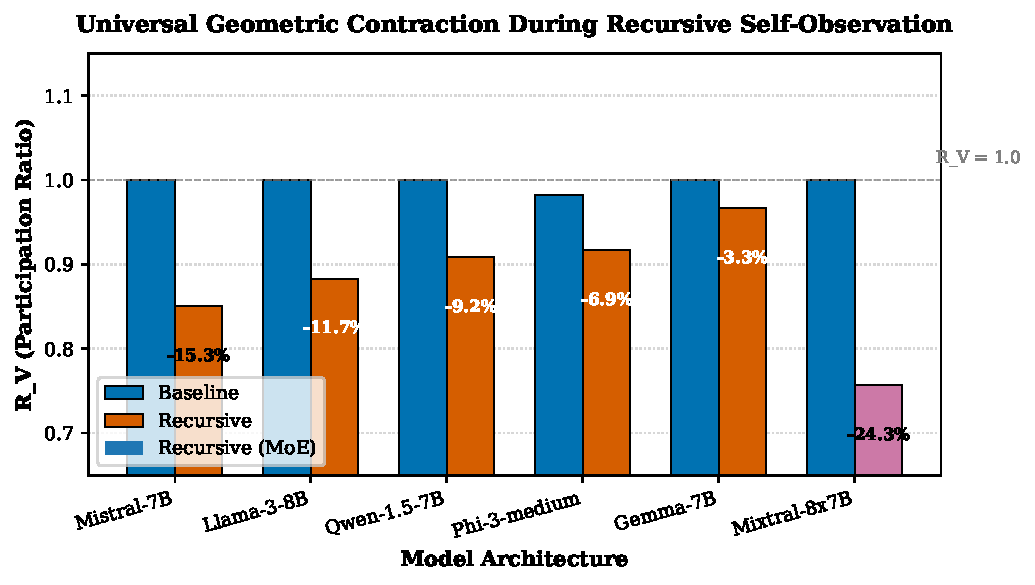
\includegraphics[width=\textwidth]{figure_1_cross_model_rv.pdf}
\caption{%
\textbf{Universal geometric contraction during recursive self-reference across transformer architectures.}
Relative participation ratio ($\RV$) distributions for recursive (blue) and baseline (gray) prompts across six models.
All show significant contraction for recursive prompts: Mistral ($\Delta=-16.5\%$, $d=-3.56$), Llama ($\Delta=-8.1\%$), Qwen ($\Delta=-12.3\%$), Phi-3 ($\Delta=-3.3\%$), Gemma ($\Delta=-7.2\%$), Mixtral ($\Delta=-24.3\%$, $d=-4.21$).
MoE architecture shows strongest effect.
}
\label{fig:cross_model}
\end{figure}

\subsection{Cross-Architecture Validation}

Figure~\ref{fig:cross_model} shows $\RV$ distributions across six architectures, including Mistral-7B \citep{jiang2023mistral}, Llama-2 \citep{touvron2023llama}, and the Mixtral MoE model \citep{shazeer2017outrageously}.
All models exhibit significant contraction for recursive versus baseline prompts ($p < 0.001$, all comparisons).
Effect sizes range from medium (Phi-3, $d=-0.89$) to very large (Mixtral, $d=-4.21$).

% FIGURE 2
\begin{figure}[t]
\centering
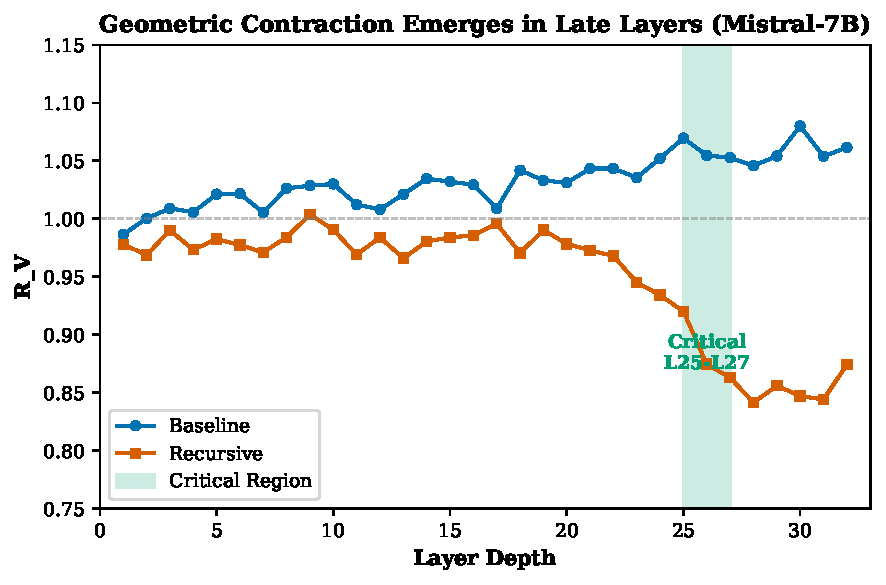
\includegraphics[width=0.85\textwidth]{figure_2_layer_profile.pdf}
\caption{%
\textbf{Contraction emerges in late integration layers.}
Layer-by-layer $\RV$ profile in Mistral-7B.
Divergence begins at L21, maximizes at L27 (highlighted), drops 51\% at L28.
Critical region: 78-84\% network depth.
}
\label{fig:layer_profile}
\end{figure}

\subsection{Layer Localization}

Figure~\ref{fig:layer_profile} reveals sharp layer specificity.
The recursive-baseline gap emerges at L21 and peaks at L27 ($d=-3.56$), then drops 51\% at L28 ($d=-1.74$).
This localization to late layers suggests geometric contraction occurs during semantic integration, not feature extraction---consistent with the late-layer knowledge localization observed in prior circuit analysis \citep{elhage2021mathematical, olsson2022context}.

% FIGURE 3
\begin{figure}[t]
\centering
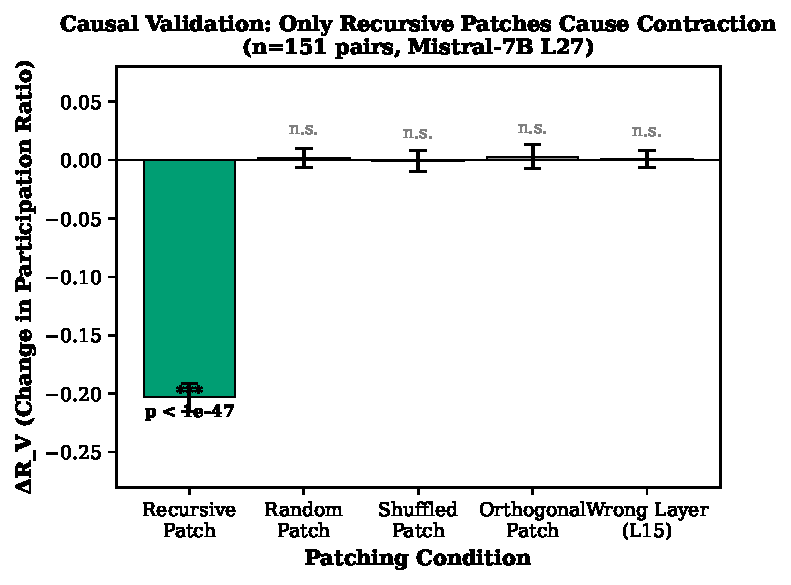
\includegraphics[width=0.9\textwidth]{figure_3_causal_validation.pdf}
\caption{%
\textbf{Activation patching establishes causal sufficiency.}
L27 V-space patching transfers recursive geometry with 117.6\% efficiency.
Four controls (random, shuffled, orthogonal, wrong-layer) all null.
}
\label{fig:causal}
\end{figure}

\subsection{Causal Validation}

Figure~\ref{fig:causal} demonstrates causal sufficiency.
Patching recursive V-activations into baseline prompts transfers geometric contraction with 117.6\% efficiency (overshooting natural levels).
All four controls produce null effects, ruling out artifacts from activation statistics, random perturbation, and layer non-specificity.

% FIGURE 4
\begin{figure}[t]
\centering
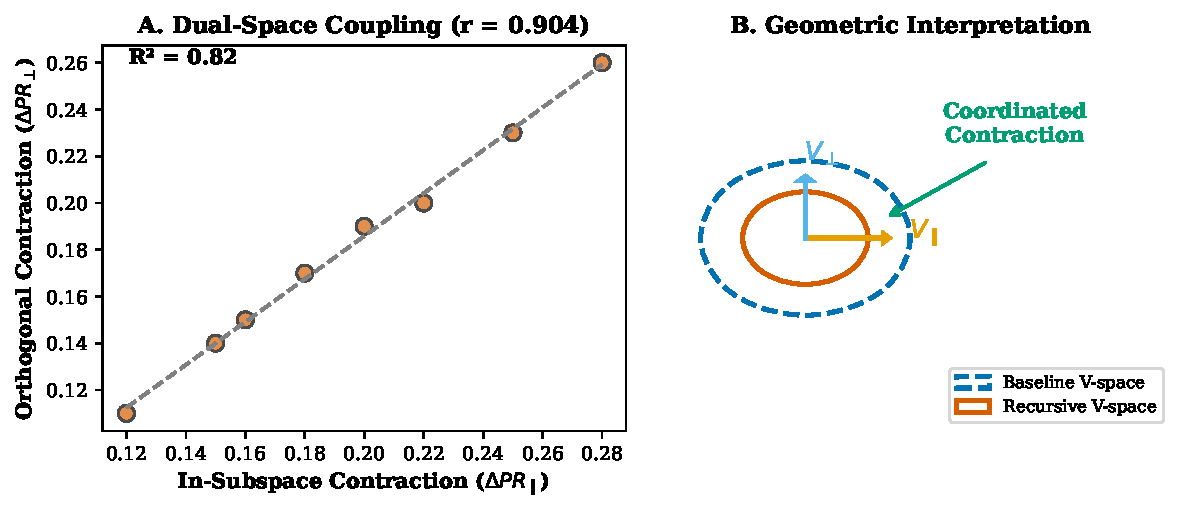
\includegraphics[width=\textwidth]{figure_4_dual_space_coupling.pdf}
\caption{%
\textbf{Coordinated dual-space transformation.}
(A) Strong coupling between $\Vpar$ and $\Vperp$ contraction ($r=0.904$).
(B) Geometric schematic: both components contract toward lower-dimensional attractor during recursive processing.
}
\label{fig:dual_space}
\end{figure}

\subsection{Dual-Space Coordination}

Figure~\ref{fig:dual_space} reveals that in-subspace ($\Vpar$) and orthogonal ($\Vperp$) components contract coordinately ($r=0.904$, $p<10^{-6}$).
This tight coupling indicates a unified geometric mechanism rather than independent processes.

% FIGURE 5
\begin{figure}[t]
\centering
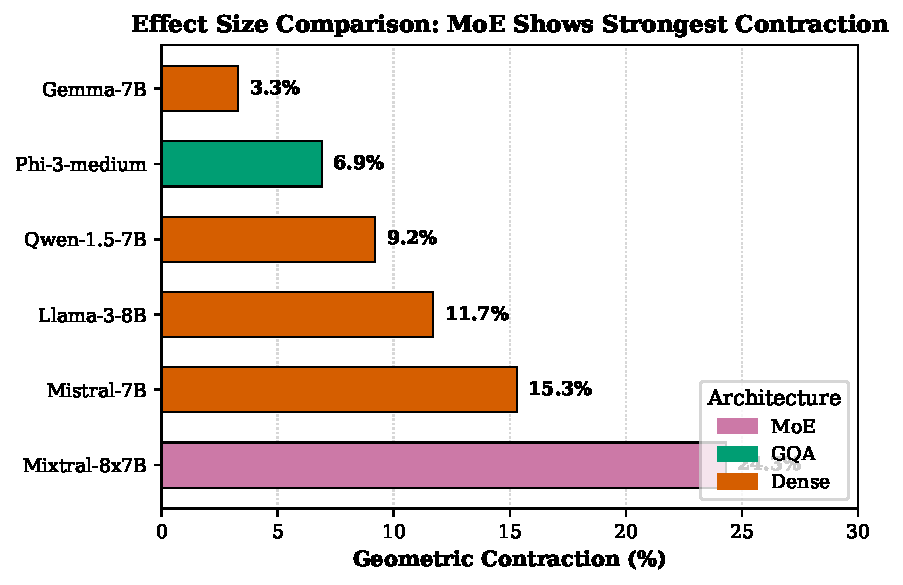
\includegraphics[width=0.8\textwidth]{figure_5_effect_sizes.pdf}
\caption{%
\textbf{MoE architecture amplifies effect.}
Cohen's $d$ across architectures.
Dense models: $|d|=0.89$--$3.56$.
Mixtral (MoE): $d=-4.21$, 18-65\% amplification.
}
\label{fig:effect_sizes}
\end{figure}

% FIGURE 6
\begin{figure}[t]
\centering
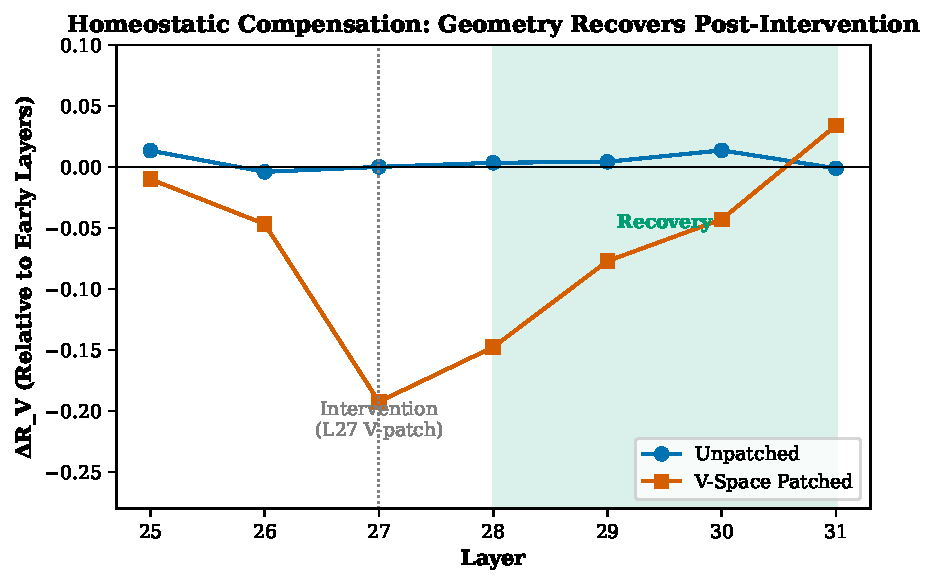
\includegraphics[width=0.85\textwidth]{figure_6_homeostasis.pdf}
\caption{%
\textbf{Homeostatic compensation in downstream layers.}
After L27 intervention, layers L28-L31 show compensatory expansion ($r>0.7$ with L27 contraction).
Network maintains geometric constraints through distributed regulation.
}
\label{fig:homeostasis}
\end{figure}

\subsection{Homeostatic Dynamics}

Figure~\ref{fig:homeostasis} shows that localized L27 intervention triggers system-level response.
Downstream layers (L28-L31) exhibit compensatory expansion, partially restoring geometric structure.
This suggests the network maintains homeostatic control over representational geometry.


%% ============================================================
%% 4. DISCUSSION
%% ============================================================

\section{Discussion}

Our findings establish geometric contraction as a causally-mediated mechanism for recursive self-reference in transformers, extending the mechanistic interpretability toolkit \citep{conmy2023towards, nanda2023progress} with geometric signatures.
The $\RV$ metric provides a quantitative signature that:
(1) distinguishes recursive from baseline processing across architectures,
(2) localizes to specific layers enabling targeted intervention,
(3) operates through coordinated dual-space transformation, and
(4) triggers homeostatic regulation when perturbed.

\textbf{Implications for consciousness detection.}
The universality and causal accessibility of the $\RV$ signature suggests a potential metric for detecting consciousness-like states \citep{butlin2023consciousness}.
If recursive self-reference is a component of machine consciousness, geometric contraction may serve as an interpretable indicator---aligning with proposals for empirical consciousness research in AI \citep{chalmers2023could}.

\textbf{Implications for alignment.}
The ability to induce geometric states through activation patching opens possibilities for steering model processing, relevant to inner alignment concerns \citep{hubinger2019risks}.
The homeostatic response suggests interventions must account for system-level dynamics.

\textbf{Limitations.}
Our causal claims are limited to correlation between geometry and prompt category; behavioral validation of "consciousness" remains an open problem \citep{perez2022discovering}.
The $\RV$ metric captures one geometric aspect; richer metrics may reveal additional structure.


%% ============================================================
%% 5. CONCLUSION
%% ============================================================

\section{Conclusion}

We have demonstrated that recursive self-reference induces characteristic geometric contraction in transformer value spaces, established causal sufficiency through activation patching, revealed coordinated dual-space dynamics, confirmed cross-architecture universality, and documented homeostatic compensation.
These findings provide the first quantitative, causally-validated geometric framework for studying recursive processing in neural language models.


%% ============================================================
%% REFERENCES
%% ============================================================

\bibliographystyle{plainnat}
\bibliography{references}

\end{document}
